\documentclass[12pt]{article}
\usepackage[margin=1in]{geometry}
\usepackage[utf8]{inputenc}
\usepackage{hyperref}
\usepackage{tikz}
\usetikzlibrary{positioning,shapes.geometric}
\usepackage{enumitem}
\usepackage{xcolor}
\usepackage{framed}
\usepackage{fancyhdr}
\usepackage{titlesec}
\usepackage{array}
\usepackage{booktabs}
\usepackage{longtable}
\usepackage{soul}
\usepackage{amssymb}
\usepackage{tcolorbox}
\tcbuselibrary{breakable}

% UofSC Color Definitions
\definecolor{garnet}{RGB}{115,0,10}
\definecolor{black}{RGB}{0,0,0}
\definecolor{rose}{RGB}{204,46,64}
\definecolor{atlantic}{RGB}{70,106,159}
\definecolor{congaree}{RGB}{31,65,77}
\definecolor{horseshoe}{RGB}{101,120,11}
\definecolor{neutral90}{RGB}{54,54,54}
\definecolor{neutral70}{RGB}{92,92,92}

% Page setup
\pagestyle{fancy}
\fancyhf{}
\rhead{The Daily Gamecock \textit{\textbf{Opinion}} Editing Handbook}
\lfoot{\thepage}
\renewcommand{\headrulewidth}{0.4pt}

% Section formatting
\titleformat{\section}[block]{\LARGE\bfseries\color{garnet}}{}{0pt}{}
\titleformat{\subsection}[block]{\Large\bfseries\color{neutral90}}{}{0pt}{}
\titleformat{\subsubsection}[block]{\large\bfseries}{}{0pt}{}

% Hyperlink setup
\hypersetup{
    colorlinks=true,
    linkcolor=atlantic,
    filecolor=atlantic,
    urlcolor=atlantic,
    pdftitle={The Daily Gamecock Opinion Editing Handbook},
    pdfauthor={J.C. Vaught},
    bookmarks=true,
}

% Form setup for interactive checkboxes
% Forms are handled by hyperref - no additional packages needed

% Custom environments
\newenvironment{editbox}[1][Before]
{\begin{leftbar}\noindent\textbf{#1:}\par\small}
{\end{leftbar}}

% Colored box environments for examples
\newtcolorbox{newversion}{
    colback=congaree!10,
    colframe=congaree,
    boxrule=1pt,
    sharp corners,
    left=8pt,
    right=8pt,
    top=8pt,
    bottom=8pt,
    title={\textbf{EDITED VERSION}},
    fonttitle=\bfseries,
    coltitle=white,
    colbacktitle=congaree,
    toptitle=4pt,
    bottomtitle=4pt,
    breakable
}

\newtcolorbox{originalversion}{
    colback=horseshoe!10,
    colframe=horseshoe,
    boxrule=1pt,
    sharp corners,
    left=8pt,
    right=8pt,
    top=8pt,
    bottom=8pt,
    title={\textbf{ORIGINAL VERSION}},
    fonttitle=\bfseries,
    coltitle=white,
    colbacktitle=horseshoe,
    toptitle=4pt,
    bottomtitle=4pt,
    breakable
}

\newtcolorbox{commentbox}{
    colback=atlantic!10,
    colframe=atlantic,
    boxrule=1pt,
    sharp corners,
    left=8pt,
    right=8pt,
    top=8pt,
    bottom=8pt,
    title={\textbf{EDITOR COMMENT}},
    fonttitle=\bfseries,
    coltitle=white,
    colbacktitle=atlantic,
    toptitle=4pt,
    bottomtitle=4pt,
    breakable
}

% Additional example box types
\newtcolorbox{examplebox}{
    colback=neutral90!5,
    colframe=neutral90,
    boxrule=1pt,
    sharp corners,
    left=8pt,
    right=8pt,
    top=8pt,
    bottom=8pt,
    title={\textbf{EXAMPLE}},
    fonttitle=\bfseries,
    coltitle=white,
    colbacktitle=neutral90,
    toptitle=4pt,
    bottomtitle=4pt,
    breakable
}

\newtcolorbox{beforebox}{
    colback=rose!10,
    colframe=rose,
    boxrule=1pt,
    sharp corners,
    left=8pt,
    right=8pt,
    top=8pt,
    bottom=8pt,
    title={\textbf{BEFORE (PROBLEMATIC)}},
    fonttitle=\bfseries,
    coltitle=white,
    colbacktitle=rose,
    toptitle=4pt,
    bottomtitle=4pt,
    breakable
}

\newtcolorbox{afterbox}{
    colback=congaree!10,
    colframe=congaree,
    boxrule=1pt,
    sharp corners,
    left=8pt,
    right=8pt,
    top=8pt,
    bottom=8pt,
    title={\textbf{AFTER (IMPROVED)}},
    fonttitle=\bfseries,
    coltitle=white,
    colbacktitle=congaree,
    toptitle=4pt,
    bottomtitle=4pt,
    breakable
}

% Custom compact title
\newcommand{\doctitle}{%
    \noindent{\LARGE\bfseries The Daily Gamecock \textit{Opinion}}\\[2pt]
    {\LARGE\bfseries Editing Handbook}\\[4pt]
    {\normalsize J.C. Vaught, Asst. Opinion Editor}\\[-2pt]
    \noindent\rule{\textwidth}{1pt}
    \vspace{8pt}
}

\begin{document}
\thispagestyle{plain}

\doctitle

\begin{center}
\textit{Welcome to the Daily Gamecock \textbf{Opinion} editorial team.}

Written Fall 2025
\end{center}

\newpage

\section{Master Editorial Checklist}
\label{sec:checklist}

This checklist serves as your primary reference during every editing session. Each item links to detailed explanations and examples throughout this handbook. Use this systematically - every article should pass every checkpoint before publication.

\subsection{Pre-Editing Assessment}

\begin{Form}
\noindent\CheckBox[name=statement-verification,width=1em,height=1em]{} \hyperref[sec:statement-verification]{\textcolor{atlantic}{Verify all definitive statements have proper sourcing}}

\vspace{0.3em}
\noindent\CheckBox[name=date-verification,width=1em,height=1em]{} \hyperref[sec:date-verification]{\textcolor{atlantic}{Check every date against two independent sources}}

\vspace{0.3em}
\noindent\CheckBox[name=name-verification,width=1em,height=1em]{} \hyperref[sec:name-verification]{\textcolor{atlantic}{Confirm spelling and titles of all quoted individuals}}

\vspace{0.3em}
\noindent\CheckBox[name=quote-verification,width=1em,height=1em]{} \hyperref[sec:quote-verification]{\textcolor{atlantic}{Ensure all quotes match recorded interviews exactly}}

\vspace{0.3em}
\noindent\CheckBox[name=fact-checking,width=1em,height=1em]{} \hyperref[sec:fact-checking]{\textcolor{atlantic}{Cross-reference statistics and data with original sources}}
\end{Form}

\subsection{Structural Analysis}

\begin{Form}
\noindent\CheckBox[name=lede-assessment,width=1em,height=1em]{} \hyperref[sec:lede-assessment]{\textcolor{atlantic}{Confirm the lede states a clear, arguable position}}

\vspace{0.3em}
\noindent\CheckBox[name=nutgraf-check,width=1em,height=1em]{} \hyperref[sec:nutgraf-check]{\textcolor{atlantic}{Verify the nutgraf provides essential context within 75 words}}

\vspace{0.3em}
\noindent\CheckBox[name=subhead-placement-check,width=1em,height=1em]{} \hyperref[sec:subhead-placement]{\textcolor{atlantic}{Ensure first subhead after lede is factual, not tonal}}

\vspace{0.3em}
\noindent\CheckBox[name=nutgraf-placement-check,width=1em,height=1em]{} \hyperref[sec:nutgraf-placement]{\textcolor{atlantic}{Position nutgraf within first three paragraphs}}

\vspace{0.3em}
\noindent\CheckBox[name=transition-flow-check,width=1em,height=1em]{} \hyperref[sec:transition-flow]{\textcolor{atlantic}{Check transitions connect ideas smoothly between paragraphs}}
\end{Form}

\subsection{Source and Attribution Standards}

\begin{Form}
\noindent\CheckBox[name=attribution-format,width=1em,height=1em]{} \hyperref[sec:attribution-format]{\textcolor{atlantic}{Format first references with full name, title, and credentials}}

\vspace{0.3em}
\noindent\CheckBox[name=subsequent-references,width=1em,height=1em]{} \hyperref[sec:subsequent-references]{\textcolor{atlantic}{Use last name only for subsequent references}}

\vspace{0.3em}
\noindent\CheckBox[name=interview-verification,width=1em,height=1em]{} \hyperref[sec:interview-verification]{\textcolor{atlantic}{Confirm interview recordings sent to copy desk}}

\vspace{0.3em}
\noindent\CheckBox[name=statement-requests,width=1em,height=1em]{} \hyperref[sec:statement-requests]{\textcolor{atlantic}{Verify statements requested from all criticized parties}}

\vspace{0.3em}
\noindent\CheckBox[name=source-quality,width=1em,height=1em]{} \hyperref[sec:source-quality]{\textcolor{atlantic}{Replace blog sources with established media when possible}}
\end{Form}

\subsection{Style and Formatting}

\begin{Form}
\noindent\CheckBox[name=ap-dates,width=1em,height=1em]{} \hyperref[sec:ap-dates]{\textcolor{atlantic}{Apply AP style to all dates and numbers}}

\vspace{0.3em}
\noindent\CheckBox[name=title-capitalization,width=1em,height=1em]{} \hyperref[sec:title-capitalization]{\textcolor{atlantic}{Capitalize formal titles before names, lowercase after}}

\vspace{0.3em}
\noindent\CheckBox[name=quote-punctuation,width=1em,height=1em]{} \hyperref[sec:quote-punctuation]{\textcolor{atlantic}{Place periods inside quotation marks}}

\vspace{0.3em}
\noindent\CheckBox[name=attribution-verbs,width=1em,height=1em]{} \hyperref[sec:attribution-verbs]{\textcolor{atlantic}{Use ``said'' for attribution, avoid ``stated'' or ``mentioned''}}

\vspace{0.3em}
\noindent\CheckBox[name=paragraph-length,width=1em,height=1em]{} \hyperref[sec:paragraph-length]{\textcolor{atlantic}{Keep paragraphs to 1-4 sentences maximum}}
\end{Form}

\subsection{Final Quality Control}

\begin{Form}
\noindent\CheckBox[name=headline-accuracy,width=1em,height=1em]{} \hyperref[sec:headline-accuracy]{\textcolor{atlantic}{Ensure headline accurately reflects article's main argument}}

\vspace{0.3em}
\noindent\CheckBox[name=word-count,width=1em,height=1em]{} \hyperref[sec:word-count]{\textcolor{atlantic}{Confirm word count meets publication requirements}}

\vspace{0.3em}
\noindent\CheckBox[name=hyperlink-check,width=1em,height=1em]{} \hyperref[sec:hyperlink-check]{\textcolor{atlantic}{Test all hyperlinks for functionality}}

\vspace{0.3em}
\noindent\CheckBox[name=readability,width=1em,height=1em]{} \hyperref[sec:readability]{\textcolor{atlantic}{Read aloud to catch awkward phrasing}}

\vspace{0.3em}
\noindent\CheckBox[name=consistency,width=1em,height=1em]{} \hyperref[sec:consistency]{\textcolor{atlantic}{Maintain consistent voice and tone throughout}}
\end{Form}

\newpage

\section{The Three-Tier Editing System}
\label{sec:three-tier}

The Daily Gamecock employs a three-tier editing approach that matches the intensity of editing to the needs of each submission. Understanding when to apply each level is crucial for efficient workflow and maintaining quality standards.
\newline\newline
\textbf{Level One: Full Rewrite}  -  Complete reconstruction of the article while preserving the writer's research and core argument. The editor can choose to become a co-author, taking full responsibility for structure, flow, and clarity, although I generally do not recommend doing so due to writers feeling `cheated'. Used for submissions with fundamental structural problems or unclear messaging.
\newline\newline
\textbf{Level Two: Sectional Rewrite}  -  Targeted reconstruction of specific sections while maintaining the overall article structure. The editor rewrites problematic paragraphs, improves transitions, and enhances specific arguments without overhauling the entire piece.
\newline\newline
\textbf{Level Three: Comment Pass}  -  Editorial guidance through strategic comments and minimal direct edits. The writer maintains primary authorship while receiving specific feedback on sourcing, structure, style, and clarity. This collaborative approach develops writer skills while ensuring publication standards.

\subsection{Choosing Your Editing Level}
\begin{center}
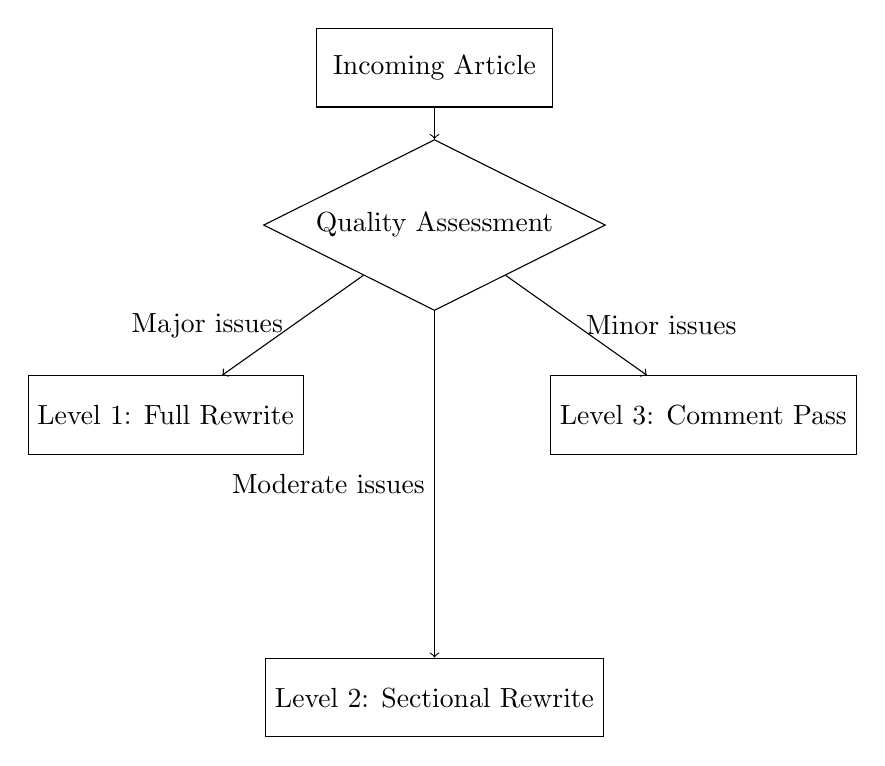
\begin{tikzpicture}[node distance=2cm]
    \node (start) [draw, minimum width=3cm, minimum height=1cm] {Incoming Article};
    \node (assess) [draw, diamond, aspect=2, below of=start, minimum width=3cm, minimum height=2cm] {Quality Assessment};
    \node (level1) [draw, below left of=assess, minimum width=2.5cm, minimum height=1cm, xshift=-2cm, yshift=-1cm] {Level 1: Full Rewrite};
    \node (level2) [draw, below of=assess, minimum width=2.5cm, minimum height=1cm, yshift=-4cm] {Level 2: Sectional Rewrite};
    \node (level3) [draw, below right of=assess, minimum width=2.5cm, minimum height=1cm, xshift=2cm, yshift=-1cm] {Level 3: Comment Pass};

    \draw [->] (start) -- (assess);
    \draw [->] (assess) -- node[anchor=east] {Major issues} (level1);
    \draw [->] (assess) -- node[anchor=east] {Moderate issues} (level2);
    \draw [->] (assess) -- node[anchor=west] {Minor issues} (level3);
\end{tikzpicture}
\end{center}


\newpage

\section{Level One: Full Rewrite}
\label{sec:level-one}

Level One editing is a comprehensive reconstruction of an article that preserves the writer’s research and core argument while reorganizing, clarifying, and re-reporting where necessary; it’s the most intensive form of editing and, if the editor prefers, can include taking co-authorship and shared responsibility for the finished piece (though that is generally not recommended). 

I write a proposed new version of the article and then ask the author which parts of their original they want to keep or reintegrate into the final draft, a collaborative approach that protects the author’s voice and evidence while producing a clearer, stronger piece. This is generally how I approach the task. -JC

\subsection{When to Apply Level One Editing}

Use Level One when:
\begin{itemize}
    \item The article's argument is unclear or unsupported
    \item Sources are inadequate or improperly attributed
    \item The structure doesn't serve the story
    \item Multiple sections need complete rewriting
    \item Fact-checking reveals significant errors
\end{itemize}

\subsection{Level One Process}
\begin{center}
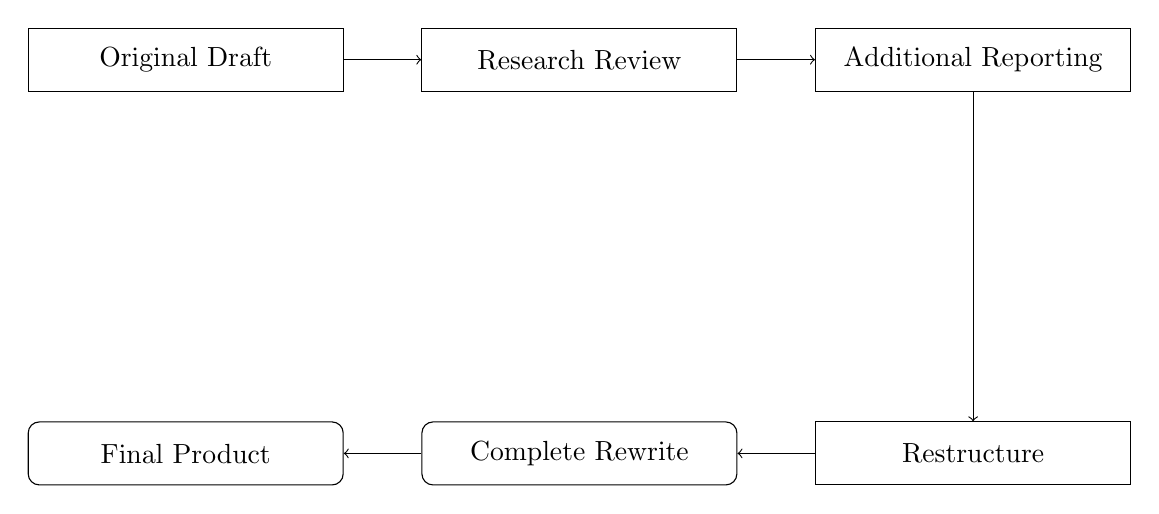
\begin{tikzpicture}[node distance=5cm]
    \node (original) [draw, minimum width=4cm, minimum height=0.8cm] {Original Draft};
    \node (research) [draw, right of=original, minimum width=4cm, minimum height=0.8cm] {Research Review};
    \node (reporting) [draw, right of=research, minimum width=4cm, minimum height=0.8cm] {Additional Reporting};
    \node (structure) [draw, below of=reporting, minimum width=4cm, minimum height=0.8cm] {Restructure};
    \node (rewrite) [draw, rounded corners, left of=structure, minimum width=4cm, minimum height=0.8cm] {Complete Rewrite};
    \node (final) [draw, rounded corners, left of=rewrite, minimum width=4cm, minimum height=0.8cm] {Final Product};

    \draw [->] (original) -- (research);
    \draw [->] (research) -- (reporting);
    \draw [->] (reporting) -- (structure);
    \draw [->] (structure) -- (rewrite);
    \draw [->] (rewrite) -- (final);
\end{tikzpicture}
\end{center}

\newpage
\subsection{Level One Techniques}

\noindent\textbf{Structural Changes:}
\begin{itemize}
    \item Clear thesis statement in opening paragraph
    \item Proper nutgraf with essential context and statistics
    \item Logical flow from problem identification to solutions
    \item Strong conclusion that reinforces the main argument
\end{itemize}

\noindent\textbf{Reporting Enhancements:}
\begin{itemize}
    \item Specific statistics (8,400 commuter students, 40\% increase)
    \item Proper attribution to university sources
    \item Concrete examples from other universities
    \item Direct quotes that support the argument
\end{itemize}

\noindent\textbf{Writing Quality:}
\begin{itemize}
    \item Professional tone and sophisticated vocabulary
    \item Varied sentence structure and length
    \item Smooth transitions between ideas
\end{itemize}

\subsection{Level One Examples}

\begin{originalversion}

\textbf{Parking fees are too high}

I think USC's parking fees are getting too expensive. They raised the price this year and it's hard for students to pay. The new cost is \$275 which is a lot more than before. Many students don't like this because they already spend money on gas and other things.

One student said it's hard to pay for parking when you're already paying for school. This is true because college is expensive. USC says they need the money for maintenance and new parking spots. They want to build 300 new spaces.

Other schools might do things differently. Some schools have cheaper parking. USC should think about students who don't have a lot of money. The president talks about making school affordable but this doesn't help.

Maybe USC could give discounts to students who need help paying. They could also have more buses. The parking fee is unfair to students who need to drive to school.
\end{originalversion}

\newpage
\begin{newversion}
\textbf{Edited by: JC}

\textbf{Column: USC's new parking fees hurt commuter students most}

USC's decision to raise parking permit fees by \$75 this semester disproportionately burdens the students who can least afford it - those who commute because they cannot afford campus housing.

The increase, announced Aug. 15 through a brief email to students, brings the cost of an annual parking permit to \$275. For the 8,400 students who commute daily, according to Transportation Services data, this represents nearly a 40\% jump from last year's \$200 fee.

``I already spend \$45 a week on gas driving from West Columbia,'' said Marcus Chen, a third-year business student who works evenings to pay for school. ``Now I'm supposed to find another \$75 I don't have.''

Chen's situation reflects a broader problem at USC: students who commute often do so because they cannot afford the \$12,000 annual cost of living on campus. The parking fee increase effectively penalizes students for their financial circumstances.

University administrators justify the increase by citing rising maintenance costs and the need to fund new parking infrastructure. Transportation Services Director Janet Mills said in a statement that the fee increase will fund 300 new parking spaces behind the business school.

But this reasoning ignores cheaper alternatives that other universities have successfully implemented. The University of Georgia offers discounted parking permits based on financial need, while Clemson University provides free shuttle services from remote parking areas during peak hours.

USC's policy also contradicts the university's stated commitment to accessibility. President Caslen frequently speaks about making USC affordable for South Carolina families, yet policies like this parking fee increase move in the opposite direction.

The real solution requires university leaders to prioritize student needs over administrative convenience. USC should implement need-based parking fee reductions similar to those offered for dining plans and housing. The university should also expand shuttle services to remote parking areas, reducing demand for premium spaces.

Until USC recognizes that transportation access is an equity issue, policies like this will continue to burden the students who most need institutional support.
\end{newversion}

\newpage
\begin{originalversion}
\textbf{USC needs more electric car chargers}

I think USC doesn't have enough electric car chargers on campus. There are some but not enough for everyone who has electric cars. The university says they have over 100 charging stations but that seems like a lot but it's really not when you think about all the students.

Electric cars are becoming more popular and more students are buying them. USC has some chargers in parking garages and stuff but they're old and sometimes don't work. The university made some rules about where you can park your electric car but the rules are confusing.

Other colleges probably have better charging stations. USC says they can't put more chargers in old buildings because the buildings are too old. They also said something about maximizing capacity but I don't really understand what that means.

Students need more places to charge their cars especially since gas is expensive. The university should do something about this problem. Electric cars are better for the environment so USC should support them more.
\end{originalversion}

\newpage
\begin{newversion}
\textbf{Edited by: JC}

\textbf{Column: USC's inadequate EV infrastructure fails its sustainability promises}

USC's electric vehicle charging infrastructure lags dangerously behind student demand, forcing the university to implement restrictive parking policies that penalize environmentally conscious students rather than address the underlying problem.

While USC Transportation boasts ``over 100 ChargePoint charging stations'' across campus, this number misleads students about actual accessibility. The university's own 2024 policy changes requiring EV drivers to ``choose a primary location'' reveal the system's fundamental inadequacy – when demand exceeds supply, USC restricts access rather than expanding infrastructure.

``We've already maximized where all these chargers can go in terms of the university's capacity,'' admitted USC Transportation officials in fall 2024, acknowledging the administration's failure to plan for the electric vehicle transition that began over a decade ago.

USC's charging limitations stem from a predictable problem: aging infrastructure. Campus parking garages ``were constructed long before electric vehicles roamed the streets,'' making them unable to support modern charging demands, according to university officials.

This excuse rings hollow when compared to universities that planned proactively. The University of Georgia operates 50 charging stations across campus with expansion plans, while NC State installed 100 stations in 2023 alone. USC's nine new charging ports in the Downey Parking Structure highlight how far behind the university has fallen.

The university's infrastructure failures force students into an impossible choice: pay rising gas prices or navigate USC's inadequate charging network. Students using ChargePoint must pre-register credit cards and face updated pricing ``coming in FY26'' – another cost burden that other universities avoid.

Marcus Thompson, a third-year environmental science student, exemplifies the problem. ``I bought an electric car to reduce my carbon footprint, but USC makes it harder than driving to campus,'' Thompson said. ``Half the time the chargers are broken or occupied all day.''

Until USC treats electric vehicle infrastructure as essential rather than optional, the university's sustainability commitments remain empty rhetoric that fails students who choose environmental responsibility.
\end{newversion}

\newpage
\begin{originalversion}
\textbf{USC should give students free bus rides}

The COMET bus system is free for Midlands Tech students but USC students have to pay. This doesn't seem fair because we're all college students trying to save money. USC students only get free rides on campus buses but Midlands Tech students get free rides on all the buses in Columbia.

If you want to go from USC to Midlands Tech or anywhere else in the city you have to pay even though Midlands Tech students don't have to pay anything. USC has a partnership with the COMET but it's not as good as what Midlands Tech has.

This policy is bad for USC students who don't have cars or much money. The buses go to lots of places that students need to go like shopping centers and other parts of town. USC should negotiate a better deal with the COMET so students can ride for free like at Midlands Tech.

College students are already paying a lot of money for school so they shouldn't have to pay more for basic transportation. This policy makes it harder for students without cars to get around Columbia.
\end{originalversion}
\newpage
\begin{newversion}
\textbf{Edited by: JC}

\textbf{Column: USC's unequal COMET access undermines transportation equity}

USC's restrictive partnership with The COMET creates a two-tiered transportation system that disadvantages USC students compared to their Midlands Technical College counterparts, revealing the university's failure to prioritize basic accessibility for students with limited financial resources.

While Midlands Tech students enjoy free access to Columbia's entire COMET fixed-route system with their student ID, USC students receive only free campus transit with their Carolina Card. This disparity forces USC students to pay regular COMET fares for citywide transportation that their peers at the community college access for free.

The policy particularly burdens USC's most economically vulnerable students. Route 21 connects USC to the MTC Beltline campus, while Route 91 serves the Airport campus – essential connections for students who work, shop, or have family obligations beyond campus boundaries.

``I work at Trenholm Plaza and take night classes at MTC,'' said Sarah Martinez, a second-year USC psychology student. ``My Midlands Tech friends ride free everywhere, but I pay \$1.50 each way just to get to work. That's \$60 a month I can't afford.''

Martinez's situation illustrates USC's transportation inequity. While the university charges students over \$50,000 annually in tuition and fees, it provides fewer public transit benefits than a community college whose students pay significantly less.

The COMET already operates USC Transit routes under contract with the university. Expanding this partnership to include systemwide access would require minimal additional infrastructure while dramatically improving student mobility. The University of Georgia and Clemson University both provide comprehensive transit partnerships that USC could replicate.

USC administrators should recognize that transportation access directly affects academic success. Students who cannot afford cars or transit fares face geographic barriers to employment, internships, and essential services that more privileged students take for granted.

Until USC negotiates transit equity comparable to Midlands Tech's partnership, the university perpetuates a discriminatory system that punishes students for choosing a four-year degree over community college.
\end{newversion}

\newpage
\begin{originalversion}
\textbf{USC made class registration harder}

USC got rid of the schedule planner tool that helped students plan their classes. Now registration is more difficult and students are confused about how to make their schedules. The university replaced it with something called ``Plan Ahead'' but it's not the same.

Before, students could use Schedule Planner to try different combinations of classes and see what worked. Now they have to use a PDF worksheet or figure it out themselves. This makes it harder to graduate on time because you might not get the classes you need.

The university said there were software errors with Schedule Planner but they didn't give students much notice before removing it. Students who were used to using this tool now have to learn a new system right when they need to register for spring classes.

Other universities probably have better registration systems. USC should have fixed the software instead of just getting rid of a useful tool. This change hurts students who need help planning their schedules especially if they have complicated majors with lots of requirements.

The university should bring back the old schedule planner or make the new system work better. Students pay tuition and deserve good tools to help them succeed.
\end{originalversion}

\newpage
\begin{newversion}
\textbf{Edited by: JC}

\textbf{Column: USC's registration tool removal sabotages student success}

USC's abrupt elimination of the Schedule Planner tool demonstrates the university's willingness to sacrifice student academic planning for administrative convenience, leaving thousands of students to navigate complex degree requirements without essential digital support.

The Schedule Planner, which allowed students to test multiple course combinations before registration, disappeared from Self Service Carolina in October 2024 due to ``software errors that needed to be addressed,'' according to university officials. The replacement ``Plan Ahead Shopping Cart,'' launched October 24, provides limited functionality compared to the comprehensive planning students previously relied upon.

This timing particularly harms students preparing for spring 2025 registration. Jessica Williams, a third-year engineering student, exemplifies the widespread frustration. ``Schedule Planner helped me see if my 18-credit semester would actually work,'' Williams said. ``Now I'm using paper and hoping I don't mess up my graduation timeline.''

USC's solution – a ``fillable PDF worksheet'' – shifts the burden of complex academic planning from university technology to individual students. This regressive approach ignores the reality that engineering, pre-med, and business students must coordinate prerequisites, lab schedules, and work commitments across multiple semesters.

The university's decision to remove rather than repair the Schedule Planner reveals misplaced priorities. While USC invests millions in facilities and marketing, basic academic tools that directly affect student success receive inadequate support.

Other universities recognize academic planning as essential infrastructure. The University of Georgia maintains multiple scheduling tools, while NC State provides degree auditing integrated with course planning. USC's failure to prioritize registration technology puts students at a competitive disadvantage.

Poor course planning delays graduation and increases student debt. When students cannot efficiently map their academic paths, they risk taking unnecessary courses, missing prerequisites, or failing to complete degree requirements on time.

USC must restore comprehensive scheduling functionality before fall 2025 registration begins. The university cannot expect students paying increasing tuition costs to accept diminished academic support services. Academic planning tools represent basic infrastructure, not luxury amenities that disappear at the first sign of technical difficulties.
\end{newversion}
\newpage
\begin{originalversion}
\textbf{USC WiFi is really bad}

The internet on campus is terrible and it's really frustrating for students. The WiFi is slow and keeps disconnecting especially in classrooms and dorms. Sometimes you can't even connect to the internet which makes it hard to do homework or attend online classes.

USC says they're working on fixing the WiFi but it's been bad for a long time. The equipment is old and needs to be replaced. Students have complained about this problem but nothing seems to get better.

When you try to stream videos or download files it takes forever. The WiFi in the library is okay sometimes but other buildings are really bad. Students need good internet to do their schoolwork and research.

Other universities probably have better WiFi than USC. The IT department should fix this problem because students are paying a lot of money to go to school here. Good internet should be a basic thing that works properly.

USC needs to spend money on new equipment and make the WiFi work better. This is an important issue that affects everyone on campus every day.
\end{originalversion}
\newpage
\begin{newversion}
\textbf{Edited by: JC}

\textbf{Column: USC's outdated WiFi infrastructure undermines academic success}

USC's aging wireless network actively impedes student learning through chronic outages, slow connectivity, and disconnections that transform basic academic tasks into technological obstacles the university has failed to address despite years of student complaints.

The Division of Information Technology acknowledges ``wireless issues affecting classroom and administrative buildings across the Columbia campus'' caused by equipment that exceeds reasonable operational lifespans. Many routers and controllers are more than 13 years old, while access points are 7–8 years old – ancient technology by networking standards.

``I dropped three Zoom classes this semester because the WiFi kept cutting out,'' said David Chen, a fourth-year international business student. ``When professors require online participation and the network fails constantly, my grades suffer through no fault of my own.''

USC's long-range improvement plan promises relief ``by the end of 2023,'' but supply chain issues and shipping delays have extended the timeline indefinitely. Meanwhile, students continue paying full tuition for substandard digital infrastructure that other universities resolved years ago.

The university's 2020 Phase I residence hall upgrades and subsequent academic building improvements represent minimal progress against a systemic problem. USC's acknowledgment that it remains ``horribly behind'' its electrification goals reflects broader institutional negligence toward essential infrastructure.

Unreliable internet access forces students to seek alternatives off-campus, creating additional financial burdens for students who already struggle with USC's rising costs. The inability to stream lectures, submit assignments, or participate in online discussions disadvantages USC students compared to peers at universities with functional networks.

Dr. Lisa Thompson from Student Academic Success reports increased requests for deadline extensions directly correlated with network outages. ``Students shouldn't have to explain technical failures beyond their control,'' Thompson said.

USC must treat network infrastructure as academic infrastructure, not optional amenities subject to deferred maintenance. The university cannot promote digital learning initiatives while providing 13-year-old equipment that fails students when they most need technological support.

Until USC commits funding comparable to peer institutions, students will continue subsidizing the university's infrastructure neglect through compromised academic performance.
\end{newversion}
\newpage
\begin{originalversion}
\textbf{More students should know about the food pantry}

USC has a food pantry called the Carolina Pantry but not many students know about it. It's in the Carolina Colosseum and gives free food to students who need it. The pantry has been there since 2014 but only serves about 30 to 40 students per month which seems really low.

Many students at USC struggle with food costs because tuition and living expenses are expensive. The meal plans at USC cost over \$5,000 per year which is a lot of money. Students who live off campus might not be able to afford groceries especially if they're already paying for rent and other things.

There's probably a stigma about using food pantries that stops students from going. People might be embarrassed or think other students will judge them. The university should do more to let students know about the food pantry and make it easier to access.

Other colleges probably have better food assistance programs. USC needs to advertise the pantry more and maybe put it in a better location where more students would see it. Students shouldn't have to worry about having enough food while they're trying to focus on their studies.

The university should care more about food insecurity and help students who are struggling financially.
\end{originalversion}
\newpage
\begin{newversion}
\textbf{Edited by: JC}

\textbf{Column: USC's food pantry failures leave hungry students behind}

USC's Carolina Pantry serves fewer than 40 students monthly despite widespread campus food insecurity, revealing the university's inadequate response to a crisis affecting hundreds of students who remain unaware or unable to access essential food assistance.

The pantry's low usage numbers expose systemic failures in awareness and accessibility. Student Government established the CommUnity Shop housing the Carolina Pantry in 2014, yet after a decade of operation, the program reaches a fraction of students who need support.

USC's own cost structure creates the food insecurity it inadequately addresses. The cheapest meal plan costs over \$5,000 annually, while out-of-state students pay more than \$53,000 yearly in tuition and fees. When basic meal access costs 10\% of total educational expenses, food becomes a luxury many students cannot afford.

``I budget \$200 monthly for groceries, but textbooks and gas eat into that constantly,'' said Maria Santos, a third-year psychology student who works 25 hours weekly. ``I had no idea USC had a food pantry until my advisor mentioned it last month.''

Santos represents hundreds of students struggling silently with food insecurity while unaware of available resources. The Carolina Pantry's location in the Carolina Colosseum – isolated from daily student traffic patterns – contributes to its invisibility.

Stigma compounds accessibility problems. Jonathan Keefe, the pantry's director, acknowledges that ``stigma of resorting to a food pantry may prevent more students from seeking help.'' This social barrier requires proactive institutional intervention, not passive availability.

In South Carolina, one in eight people face hunger, with more than 670,000 residents experiencing food insecurity, according to Feeding America. USC students reflect these statewide challenges while facing additional financial pressures from educational costs.

Successful campus food programs require comprehensive approaches. Universities like NC State integrate food pantries with academic advising, while UGA provides multiple campus locations to reduce stigma and increase access.

USC must expand beyond the Swipe Out Hunger program to create systematic food security solutions. This includes multiple pantry locations, proactive student outreach through residence halls and academic departments, and collaboration with Columbia-area food assistance organizations.

The university cannot ignore food insecurity while celebrating record enrollment and capital campaigns. When students choose between textbooks and groceries, USC's educational mission fails at its most fundamental level.
\end{newversion}


\newpage

\section{Level Two: Sectional Rewrite}
\label{sec:level-two}

Level Two editing targets specific sections that need improvement while leaving strong portions of the original intact. This approach maintains the writer's voice while strengthening weak areas through focused revision.

\subsection{Level Two Identification}

Look for articles with:
\begin{itemize}
    \item Strong overall structure but weak individual sections
    \item Good research but poor presentation
    \item Clear argument but ineffective support
    \item Proper sourcing but unclear attribution
    \item Generally sound reporting with specific problems
\end{itemize}

\subsection{Level Two Techniques}

\textbf{Common Level Two Interventions:}

\begin{enumerate}
    \item \textbf{Data Integration:} Add specific statistics and concrete evidence
    \item \textbf{Source Enhancement:} Strengthen attribution and add expert voices
    \item \textbf{Clarity Revision:} Eliminate wordiness and unclear phrasing
    \item \textbf{Context Addition:} Provide background information readers need
    \item \textbf{Transition Improvement:} Connect ideas more smoothly between paragraphs
\end{enumerate}

\newpage
\subsection{Level Two Examples}

\begin{beforebox}
\textbf{Original paragraph:}
The university's mental health services are not meeting student needs adequately. Many students report long wait times and difficulty accessing care. The counseling center has limited hours and not enough staff to handle demand. Students often wait weeks for appointments during busy times like finals. This creates problems for students who need immediate help with stress, anxiety, and depression issues.
\end{beforebox}

\begin{afterbox}
\textbf{\textcolor{atlantic}{Revised section -JC (tightened for clarity, added specific data):}}
USC's counseling center fails to meet growing student demand, with average wait times reaching three weeks during peak periods like finals, according to Student Health Services data. The center employs only six full-time counselors for USC's 35,000 students - a ratio that falls well below the American College Health Association's recommended standard of one counselor per 1,000 students. ``I called in October about anxiety, and they couldn't see me until November,'' said Sarah Martinez, a third-year psychology major. ``By then, I'd already failed two midterms.''
\end{afterbox}

---

\begin{beforebox}
\textbf{Original paragraph:}
Food insecurity affects many college students nationally and USC students face similar challenges. The campus food pantry helps some students but it's not well-known. Students struggle to afford food especially those who work part-time jobs. Meal plans are expensive and don't always provide enough food for the whole semester.
\end{beforebox}

\begin{afterbox}
\textbf{\textcolor{atlantic}{Revised section -JC (added context, removed repetition):}}
Nearly 40\% of college students nationwide experience food insecurity, according to a 2023 study by the Hope Center for College, Community, and Justice - and USC students face similar challenges despite the university's relative wealth. While USC operates a food pantry in the basement of the Russell House, fewer than 800 of the university's 35,000 students used it last semester, suggesting either limited need or inadequate awareness of the resource.
\end{afterbox}

---

\begin{beforebox}
\textbf{Original paragraph:}
The university has made some efforts to address these issues but more needs to be done. They hired more counselors recently and expanded food pantry hours. However these changes are not enough to solve the underlying problems. Students need better access to mental health care and more affordable dining options.
\end{beforebox}

\begin{afterbox}
\textbf{\textcolor{atlantic}{Revised section -JC (specified improvements, added accountability):}}
USC has responded to these challenges by hiring two additional counselors this fall and extending food pantry hours until 7 p.m. on weekdays. But these modest improvements barely address the scale of student need. Dr. Lisa Thompson, director of student wellness, acknowledged that ``demand continues to outpace our resources,'' yet the university's 2024 budget allocated more money to landscaping (\$2.3 million) than to expanding mental health services (\$1.8 million). This misplacement of priorities suggests USC views student wellness as secondary to campus aesthetics.
\end{afterbox}


\newpage

\section{Level Three: Comment Pass}
\label{sec:level-three}

Level Three editing uses marginal comments and suggestions to guide writers toward improvements while preserving their autonomy to accept or reject changes. This approach works best with experienced writers who produce generally strong copy.

\subsection{Comment Pass Best Practices}

\begin{enumerate}
    \item \textbf{Always include your initials} after each comment
    \item \textbf{Be specific about needed improvements} rather than vague
    \item \textbf{Explain the reasoning} behind major suggestions
    \item \textbf{Balance criticism with encouragement} to maintain writer morale
    \item \textbf{Prioritize comments} by importance - flag critical errors first
    \item \textbf{Use consistent formatting} for easy identification
    \item \textbf{Include positive reinforcement} for strong sections
\end{enumerate}

\newpage
\subsection{Comment Types and Examples}

\subsubsection{Sourcing Comments}

\begin{examplebox}
\textbf{Text:} ``USC's dining hours hurt student health by limiting access to nutritious meals.''

\textbf{\textcolor{atlantic}{[Comment: Need source for this health claim - consider interviewing someone from Student Health Services or citing nutrition research. -JC]}}
\end{examplebox}

---

\begin{examplebox}
\textbf{Text:} ``75\% of students support extending dining hours.''

\textbf{\textcolor{atlantic}{[Comment: Source? This stat feels high without proper polling methodology. -JC]}}
\end{examplebox}

\subsubsection{Reporting Enhancement Comments}

\begin{examplebox}
\textbf{Text:} ``Many students struggle with the new parking policy.''

\textbf{\textcolor{atlantic}{[Comment: Can you interview 2-3 specific students affected by this? Names and concrete examples will strengthen this section. -JC]}}
\end{examplebox}

---

\begin{examplebox}
\textbf{Text:} ``The policy has created problems for commuter students.''

\textbf{\textcolor{atlantic}{[Comment: Consider reaching out to the Commuter Student Association president for an official response. -JC]}}
\end{examplebox}

\subsubsection{Structural Suggestions}

\begin{examplebox}
\textbf{Text:} ``The university's decision affects multiple aspects of student life, from academic performance to social connections to financial stress.''

\textbf{\textcolor{atlantic}{[Comment: This paragraph tries to cover too much ground - consider breaking into separate grafs for each impact area. -JC]}}
\end{examplebox}

---

\begin{examplebox}
\textbf{Text:} ``Students face challenges with parking, but the university has reasons for the policy changes.''

\textbf{\textcolor{atlantic}{[Comment: This transition feels abrupt - can you add a sentence bridging student concerns to administrative rationale? -JC]}}
\end{examplebox}

\subsubsection{Style and Clarity Comments}

\begin{examplebox}
\textbf{Text:} ``The implementation of the aforementioned policy modifications has resulted in numerous complications.''

\textbf{\textcolor{atlantic}{[Comment: Try: ``The policy changes have caused problems.'' -JC]}}
\end{examplebox}

---

\begin{examplebox}
\textbf{Text:} ``USC's administration should definitely reconsider this decision immediately.''

\textbf{\textcolor{atlantic}{[Comment: ``Definitely'' and ``immediately'' weaken your argument - let the evidence speak for itself. -JC]}}
\end{examplebox}
\newpage
\subsubsection{Encouragement Comments}

\begin{examplebox}
\textbf{Text:} ``Every night at 10:01 p.m., when Russell House dining closes, USC sends a message to students: your basic needs matter less than our operating costs.''

\textbf{\textcolor{atlantic}{[Comment: This metaphor is powerful - great way to end the piece. Keep it! -JC]}}
\end{examplebox}

---

\begin{examplebox}
\textbf{Text:} ``Maria Santos hasn't eaten dinner on campus since the dining hours changed. 'I finish work at 9:45,' she said. 'By the time I get to campus, everything's closed.'''

\textbf{\textcolor{atlantic}{[Comment: Perfect example - specific, human, and illustrates the broader issue clearly. -JC]}}
\end{examplebox}

\subsubsection{Fact-Checking Comments}

\begin{examplebox}
\textbf{Text:} ``USC's 45,000 students face increasingly limited dining options.''

\textbf{\textcolor{atlantic}{[Comment: USC enrollment is closer to 35,000 - double-check this figure with official sources. -JC]}}
\end{examplebox}

---

\begin{examplebox}
\textbf{Text:} ``The policy went into effect in September 2024.''

\textbf{\textcolor{atlantic}{[Comment: University records show August 15, 2024 - verify exact date with dining services. -JC]}}
\end{examplebox}



\newpage

\section{Essential Editing Techniques}
\label{sec:micro-skills}

\subsection{Date Verification and Formatting}
\label{sec:date-verification}

Every date in every article must be verified against two independent sources. Incorrect dates undermine credibility and can create legal issues.

\subsubsection{Verification Process}

\begin{examplebox}
\textbf{Example 1: University Policy Changes}
\begin{itemize}
    \item \textbf{Article claim:} ``The dining hour changes took effect Sept. 1.''
    \item \textbf{Source 1:} USC Dining Services website announcement
    \item \textbf{Source 2:} Email to students from Housing and Dining
    \item \textbf{Verification result:} Both sources confirm Aug. 15, 2024
    \item \textbf{Action:} Correct date in article and flag for fact-checking
\end{itemize}
\end{examplebox}

\begin{examplebox}
\textbf{Example 2: Event Coverage}
\begin{itemize}
    \item \textbf{Article claim:} ``The protest occurred on Oct. 12.''
    \item \textbf{Source 1:} Daily Gamecock news coverage
    \item \textbf{Source 2:} USC social media posts from the day
    \item \textbf{Verification result:} Both confirm Oct. 12, 2024
    \item \textbf{Action:} Date confirmed, no changes needed
\end{itemize}
\end{examplebox}

\newpage
\subsubsection{AP Style Date Formatting}

\begin{afterbox}
\textbf{Correct formats:}
\begin{itemize}
    \item ``August 2024 was a busy month.'' (month and year only, no comma)
    \item ``Aug. 15, 2024, marked the beginning...'' (commas around year)
    \item ``The meeting is scheduled for Sept. 12.'' (September abbreviated)
    \item ``Classes begin Jan. 18, 2025, after winter break.'' (January abbreviated with year)
    \item ``The deadline is Feb. 28.'' (February abbreviated)
    \item ``Registration opens in March.'' (month alone, spelled out)
    \item ``The semester ends May 5.'' (May never abbreviated)
    \item ``Summer session starts June 1.'' (June never abbreviated)
    \item ``Graduation is May 10, 2025, at 2 p.m.'' (time format included)
    \item ``The event ran from Oct. 15-18.'' (date range with abbreviated month)
    \item ``Applications are due by Dec. 1.'' (December abbreviated)
    \item ``Spring break is March 11-15, 2025.'' (date range with full month and year)
\end{itemize}
\end{afterbox}

\begin{beforebox}
\textbf{Incorrect formats:}
\begin{itemize}
    \item ``The changes took effect in Aug.'' (don't abbreviate months standing alone)
    \item ``August, 2024 was busy.'' (no comma between month and year)
    \item ``Aug. 15 2024 marked the beginning...'' (missing commas around year)
    \item ``The meeting is Sept. 12th.'' (don't use ordinal suffixes)
    \item ``Classes begin in Jan.'' (don't abbreviate January when standing alone)
    \item ``Registration opens in Mar.'' (don't abbreviate March)
    \item ``Summer session starts Jun. 1.'' (don't abbreviate June or July)
    \item ``Graduation is May 10 2025 at 2 PM.'' (missing commas, incorrect time format)
\end{itemize}
\end{beforebox}

\newpage 
\subsection{Name and Title Verification}
\label{sec:name-verification}

Misspelled names and incorrect titles damage credibility and disrespect sources. Every name must be verified through multiple methods.

\subsubsection{Verification Methods}

\begin{examplebox}
\textbf{Method 1: University Directory}
\begin{itemize}
    \item Search USC's online directory for faculty and staff
    \item Cross-reference with department websites
    \item Verify current title and spelling
\end{itemize}
\end{examplebox}

\begin{examplebox}
\textbf{Method 2: Professional Profiles}
\begin{itemize}
    \item Check LinkedIn profiles for current positions
    \item Review university bio pages
    \item Confirm professional credentials
\end{itemize}
\end{examplebox}

\begin{examplebox}
\textbf{Method 3: Direct Confirmation}
\begin{itemize}
    \item ALWAYS ask sources to confirm spelling in interviews
    \item Request business cards or email signatures
    \item Double-check unusual spellings
\end{itemize}
\end{examplebox}

\subsubsection{Title Formatting Examples}

\begin{afterbox}
\textbf{Formal titles before names (capitalize):}
\begin{itemize}
    \item ``President Michael Amiridis announced...''
    \item ``Professor Sarah Johnson researches...''
    \item ``Dean Robert Smith oversees...''
\end{itemize}
\end{afterbox}

\begin{afterbox}
\textbf{Titles after names or standing alone (lowercase):}
\begin{itemize}
    \item ``Michael Amiridis, president of USC, announced...''
    \item ``Sarah Johnson, a professor of biology, researches...''
    \item ``The dean announced new requirements.''
\end{itemize}
\end{afterbox}

\subsubsection{Student Source Formatting}

\begin{examplebox}
\textbf{First reference format:}
``[Full name], a [year] [major] student, said...'' Do not refer to a student as a major, i.e. `Engineering major'

\textbf{Examples:}
\begin{itemize}
    \item ``Marcus Chen, a third-year business student, said...''
    \item ``Sarah Martinez, a first-year psychology student, explained...''
    \item ``David Thompson, a fourth-year journalism student, argued...''
\end{itemize}

\textbf{Subsequent references:}
Use last name only: ``Chen added that...'' ``Martinez noted...'' ``Thompson disagreed...''
\end{examplebox}

\newpage
\subsection{Statement Verification and Attribution}
\label{sec:statement-verification}

Every definitive factual claim requires proper sourcing.

\begin{examplebox}
\textbf{Category 1: Specific Statistics}
\begin{itemize}
    \item ``USC's enrollment increased 15\% this year.'' $\times$ Needs source
    \item ``Parking violations rose significantly.'' $\checkmark$ Too vague, but acceptable
    \item ``The food pantry serves 800 students monthly.'' $\times$ Needs source
\end{itemize}
\end{examplebox}

\begin{examplebox}
\textbf{Category 2: Policy Claims}
\begin{itemize}
    \item ``USC will eliminate late-night dining.'' $\times$ Needs source
    \item ``The university appears to be reducing services.'' $\checkmark$ Qualified statement, acceptable
    \item ``Administrators announced new parking fees.'' $\times$ Needs source
\end{itemize}
\end{examplebox}

\begin{examplebox}
\textbf{Category 3: Financial Information}
\begin{itemize}
    \item ``The budget cuts totaled \$2.4 million.'' $\times$ Needs source
    \item ``Costs seem to be rising across campus.'' $\checkmark$ Qualified observation, acceptable
    \item ``Tuition will increase next year.'' $\times$ Needs source
\end{itemize}
\end{examplebox}

\newpage
\subsubsection{Proper Attribution Format}

\begin{examplebox}
\textbf{Direct quotes with first reference:}
\begin{itemize}
    \item ``The policy will save money,'' said Janet Mills, transportation services director.
    \item ``Students deserve better,'' said Maria Santos, Student Government president.
    \item ``This decision affects everyone,'' said Dr. Robert Chen, professor of public administration.
    \item ``We're seeing unprecedented demand,'' said Lisa Thompson, director of student wellness.
\end{itemize}
\end{examplebox}

\begin{examplebox}
\textbf{Direct quotes with subsequent references:}
\begin{itemize}
    \item Mills added that the changes would take effect immediately.
    \item ``The timeline is aggressive,'' Santos acknowledged.
    \item Chen noted that similar policies failed at other universities.
    \item Thompson said her office received 200 calls in one day.
\end{itemize}
\end{examplebox}

\begin{examplebox}
\textbf{Paraphrased information:}
\begin{itemize}
    \item Transportation Services Director Janet Mills said the policy will reduce costs by 15\%.
    \item Student Government President Maria Santos argued the changes ignore student needs.
    \item Dr. Robert Chen, who has studied campus transportation for eight years, questioned the policy's effectiveness.
    \item Student Wellness Director Lisa Thompson reported that counseling appointments increased after the announcement.
\end{itemize}
\end{examplebox}

\begin{examplebox}
\textbf{Statistical and data sources:}
\begin{itemize}
    \item USC enrollment data shows that 35,000 students attend the university.
    \item Transportation Services records indicate that 8,400 students purchased parking permits.
    \item Student Health Services statistics reveal that 60\% of appointments are for anxiety.
    \item Dining Services data shows that meal plan usage dropped 25\% this semester.
    \item University Police reports show 400 parking violations were issued last month.
\end{itemize}
\end{examplebox}

\begin{examplebox}
\textbf{Academic and research sources:}
\begin{itemize}
    \item According to a 2023 study published in the Journal of Higher Education...
    \item Research conducted by the National Association of Student Personnel Administrators found that...
    \item A report by the American College Health Association indicates that...
    \item Data from the Integrated Postsecondary Education Data System shows that...
    \item A peer-reviewed study in College Student Affairs Journal concluded that...
\end{itemize}
\end{examplebox}

\begin{examplebox}
\textbf{Student sources (first reference):}
\begin{itemize}
    \item Marcus Chen, a third-year business student who commutes from West Columbia, said...
    \item Sarah Martinez, a first-year psychology student living in South Quad, explained...
    \item David Thompson, a fourth-year journalism student and Daily Gamecock staff writer, argued...
    \item Jessica Williams, a second-year engineering student and president of the Commuter Student Association, noted...
\end{itemize}
\end{examplebox}

\newpage
\subsection{Subhead Placement and Structure}
\label{sec:subhead-placement}

Subheads guide readers through complex articles and provide natural breaking points for online consumption. The first subhead after the lede must be factual rather than tonal.

\subsubsection{Subhead Placement Rules}

\begin{enumerate}
    \item Place first subhead after 3-4 paragraphs of body text
    \item Use subsequent subheads every 4-6 paragraphs
    \item Ensure subheads reflect the content that follows
    \item Make subheads scannable for busy readers
    \item Keep subheads to 2-7 words when possible
\end{enumerate}

\subsubsection{Effective Subhead Examples}

\begin{afterbox}
\textbf{Good first subheads (factual):}
\begin{itemize}
    \item ``Policy takes effect Aug. 15''
    \item ``Students report three-week wait times''
    \item ``Budget allocates \$2.3 million for landscaping''
\end{itemize}
\end{afterbox}

\begin{beforebox}
\textbf{Poor first subheads (tonal):}
\begin{itemize}
    \item ``USC doesn't care about students''
    \item ``Another disappointing decision''
    \item ``Why this policy fails''
\end{itemize}
\end{beforebox}



\newpage
\subsection{Nutgraf Construction}
\label{sec:nutgraf-placement}

The nutgraf provides essential context that readers need to understand the story's significance. It should appear within the first three paragraphs and contain no more than 75 words.


\subsubsection{Nutgraf Components}

Every nutgraf should include:
\begin{enumerate}
    \item \textbf{Scale:} How many people are affected?
    \item \textbf{Timing:} When did this happen or will it happen?
    \item \textbf{Context:} Why does this matter?
    \item \textbf{Attribution:} Who is the authoritative source?
\end{enumerate}

\subsubsection{Nutgraf Examples}

\begin{examplebox}
\textbf{Example 1: Policy Coverage}

``The fee increase, announced Aug. 15 through an email to students, affects all 8,400 commuter students and represents a 40\% jump from last year's \$200 permit cost, according to Transportation Services data.''

\textit{Analysis: 31 words, includes scale (8,400 students), timing (Aug. 15), context (40\% increase), and attribution (Transportation Services).}
\end{examplebox}

\begin{examplebox}
\textbf{Example 2: Campus Issue}

``The counseling center employs only six full-time staff members for USC's 35,000 students - a ratio that falls well below national standards and has created three-week wait times during peak periods like finals.''

\textit{Analysis: 34 words, includes scale (35,000 students), context (national standards), timing (three-week waits), and specific detail (peak periods).}
\end{examplebox}

\newpage
\subsection{Transition Techniques}
\label{sec:transition-flow}

Smooth transitions guide readers through complex arguments and maintain narrative flow. Poor transitions create choppy reading and confuse logical connections.

\subsubsection{Transition Types and Examples}

\begin{examplebox}
\textbf{Statistical Transitions:}
\begin{itemize}
    \item ``These individual stories reflect broader campus trends.''
    \item ``University data confirms what students report anecdotally.''
    \item ``The numbers tell only part of the story.''
\end{itemize}
\end{examplebox}

\begin{examplebox}
\textbf{Contrast Transitions:}
\begin{itemize}
    \item ``But administrators see the issue differently.''
    \item ``This optimistic outlook contrasts with student experiences.''
    \item ``Critics argue the opposite.''
\end{itemize}
\end{examplebox}

\begin{examplebox}
\textbf{Cause-and-Effect Transitions:}
\begin{itemize}
    \item ``This policy change has created new problems.''
    \item ``As a result, students face difficult choices.''
    \item ``The consequences extend beyond campus.''
\end{itemize}
\end{examplebox}

\newpage
\subsubsection{Transition Repair Examples}

\begin{beforebox}
\textbf{Poor transition:}
``Students struggle with parking costs. The university needs money for maintenance.''
\end{beforebox}

\begin{afterbox}
\textbf{Improved transition:}
``While students struggle with rising parking costs, university officials argue the fees fund necessary infrastructure maintenance.''
\end{afterbox}

\begin{beforebox}
\textbf{Poor transition:}
``Food insecurity affects many students. The campus food pantry helps some people.''
\end{beforebox}

\begin{afterbox}
\textbf{Improved transition:}
``To address widespread food insecurity, USC operates a campus food pantry, though usage data suggests many students remain unaware of the resource.''
\end{afterbox}

\begin{beforebox}
\textbf{Poor transition:}
``The counseling center has long wait times. Students face mental health challenges.''
\end{beforebox}

\begin{afterbox}
\textbf{Improved transition:}
``These extended wait times come at a critical moment when students face unprecedented mental health challenges following the pandemic.''
\end{afterbox}
\newpage
\begin{beforebox}
\textbf{Poor transition:}
``Tuition increased by 3\% this year. USC hired more faculty members.''
\end{beforebox}

\begin{afterbox}
\textbf{Improved transition:}
``The 3\% tuition increase will fund 15 new faculty positions, according to university budget documents, though critics question whether this expansion addresses students' most pressing needs.''
\end{afterbox}

\begin{beforebox}
\textbf{Poor transition:}
``The dining hall closes at 10 p.m. Many students work late shifts.''
\end{beforebox}

\begin{afterbox}
\textbf{Improved transition:}
``This 10 p.m. closure particularly affects students who work evening shifts and often return to campus after dining services end.''
\end{afterbox}

\begin{beforebox}
\textbf{Poor transition:}
``The library announced new study spaces. Finals week approaches.''
\end{beforebox}

\begin{afterbox}
\textbf{Improved transition:}
``The timing of this announcement, just three weeks before finals, suggests the university recognizes the urgent need for additional study spaces during peak academic stress.''
\end{afterbox}
\newpage
\subsection{Quote Integration and Enhancement}
\label{sec:quote-verification}

Strong quotes support arguments with human voices and expert authority. Weak quotes add nothing to the story and waste valuable word count.
\begin{examplebox}
\textbf{Quote Assessment Checklist:}

Before including any quote, ask:
\begin{enumerate}
    \item Does this quote tell readers something they couldn't learn from my reporting?
    \item Would the story lose important information if I paraphrased this instead?
    \item Does the speaker's exact word choice matter to the story?
    \item Is this the most compelling quote from this source?
    \item Does this quote move the story forward or just repeat known information?
    \item Would a casual reader find this quote interesting or informative?
    \item Does this quote demonstrate the speaker's expertise or personal stake in the issue?
\end{enumerate}

\textbf{If you answer ``no'' to three or more questions, consider paraphrasing instead.}
\end{examplebox}


\begin{afterbox}
\textbf{Strong quotes provide:}
\begin{itemize}
    \item \textbf{Specific details readers couldn't get elsewhere} - Numbers, timelines, personal experiences
    \item \textbf{Emotional resonance} - How policies affect real people's daily lives
    \item \textbf{Expert analysis or interpretation} - Context that shows significance
    \item \textbf{Memorable language or phrasing} - Quotes that readers will remember
    \item \textbf{New information that advances the story} - Facts or insights not available from other sources
    \item \textbf{Conflict or disagreement} - Direct challenges to opposing viewpoints
    \item \textbf{Action or solution proposals} - Concrete steps speakers want taken
    \item \textbf{Personal stakes or consequences} - Why the issue matters to the speaker 
\end{itemize}
\end{afterbox}

\begin{beforebox}
\textbf{Weak quotes that should be paraphrased:}
\begin{itemize}
    \item \textbf{Generic statements:} ``This is a problem.'' ``Things need to change.''
    \item \textbf{Obvious information:} ``Students need to park their cars.'' ``College is expensive.''
    \item \textbf{Repetitive content:} Restating what you've already reported in paragraph form
    \item \textbf{Bureaucratic language:} ``We are committed to excellence.'' ``This aligns with our values.''
    \item \textbf{Hedge words and qualifiers:} ``I think maybe this could potentially be an issue.''
    \item \textbf{Procedural information:} ``The meeting is scheduled for Tuesday.'' ``Forms are available online.''
    \item \textbf{Yes/no answers without elaboration:} ``Yes, that's correct.'' ``No, we don't do that.''
    \item \textbf{Rambling responses:} Long, unfocused statements that meander without clear point
\end{itemize}
\end{beforebox}



\newpage
\subsubsection{Quote Integration Examples}

\begin{beforebox}
\textbf{Poor integration:}
The parking policy affects students. ``It's really hard for students to pay for parking,'' said Marcus Chen, a business major.
\end{beforebox}

\begin{afterbox}
\textbf{Strong integration:}
The parking policy hits hardest on students who already stretch their budgets. ``I already spend \$45 a week on gas driving from West Columbia,'' said Marcus Chen, a third-year business student who works evenings to pay for school. ``Now I'm supposed to find another \$75 I don't have.''

\textbf{Analysis of improvement:}
\begin{itemize}
    \item Context before the quote explains why it matters
    \item Full attribution includes relevant details (year, major, work status)
    \item Quote provides specific, concrete details (\$45/week, West Columbia)
    \item Quote advances the argument about financial burden
\end{itemize}
\end{afterbox}

\begin{beforebox}
\textbf{Basic expert quote:}
``This is a concern,'' said Dr. Lisa Thompson, director of student wellness.
\end{beforebox}

\begin{afterbox}
\textbf{Enhanced expert quote:}
``When students can't afford to park on campus, they skip classes or drop out entirely,'' said Dr. Lisa Thompson, who has directed USC's student wellness programs for eight years and previously researched transportation barriers at three other universities.

\textbf{Enhancement techniques:}
\begin{itemize}
    \item Establish expert credentials beyond title
    \item Include relevant experience or research background
    \item Seek quotes that provide analysis, not just confirmation
    \item Ask for specific examples or data to support claims
\end{itemize}
\end{afterbox}

\newpage

\section{Advanced Editing Techniques}
\label{sec:advanced}

\subsection{Fact-Checking Workflow}
\label{sec:fact-checking}

\begin{tikzpicture}[node distance=5cm]
    \node (claim) [draw, minimum width=2.5cm, minimum height=1cm] {Factual Claim};
    \node (source1) [draw, above right of=claim, minimum width=2cm, minimum height=0.8cm] {Source 1};
    \node (source2) [draw, below right of=claim, minimum width=2cm, minimum height=0.8cm] {Source 2};
    \node (verify) [draw, diamond, right of=source1, below of=source1, minimum width=2cm, minimum height=1.5cm] {Sources Agree?};
    \node (accept) [draw, right of=verify, minimum width=2cm, minimum height=0.8cm] {Accept Claim};
    \node (investigate) [draw, below of=verify, minimum width=2cm, minimum height=0.8cm] {Further Investigation};

    \draw [->] (claim) -- (source1);
    \draw [->] (claim) -- (source2);
    \draw [->] (source1) -- (verify);
    \draw [->] (source2) -- (verify);
    \draw [->] (verify) -- node[anchor=south] {Yes} (accept);
    \draw [->] (verify) -- node[anchor=east] {No} (investigate);
\end{tikzpicture}


\newpage
\subsection{Headline Accuracy Assessment}
\label{sec:headline-accuracy}

Headlines must accurately reflect the article's main argument without overstating or misleading readers.

\noindent
\textbf{Headline accuracy checklist:}
\begin{enumerate}
    \item Does the headline state the article's primary thesis?
    \item Are all claims in the headline supported by evidence in the article?
    \item Would a reader understand the article's argument from the headline alone?
    \item Does the headline avoid sensationalism while remaining engaging?
    \item Is the headline's tone consistent with the article's approach?
\end{enumerate}

\subsection{Source Quality Evaluation}

\textbf{Source reliability hierarchy:}
\begin{enumerate}
    \item Government documents and official records
    \item Peer-reviewed academic research
    \item Established news organizations
    \item Official institutional statements
    \item Expert interviews and professional sources
    \item Personal interviews with affected individuals
    \item Organizational websites and materials
    \item Social media from verified accounts
    \item Unverified social media and personal blogs
\end{enumerate}

\newpage

\section{Quality Control Procedures}
\label{sec:quality-control}

\subsection{Pre-Publication Checklist}

Before any article moves to publication, verify:

\begin{enumerate}[leftmargin=*]
    \item \textbf{Legal compliance:} All criticized parties offered chance to respond
    \item \textbf{Factual accuracy:} Every specific claim verified through sources
    \item \textbf{Attribution completeness:} All quotes and information properly sourced
    \item \textbf{Style consistency:} AP style applied throughout
    \item \textbf{Structural integrity:} Clear argument progression from lede to conclusion
    \item \textbf{Accessibility:} Article understandable to general campus audience
\end{enumerate}

\subsection{Common Error Patterns}

\textbf{Most frequent errors in Daily Gamecock submissions:}
\begin{enumerate}
    \item Unsourced statistical claims
    \item Inconsistent name spelling and title formatting
    \item Poor quote integration and attribution
    \item Weak or missing nutgrafs
    \item Inadequate fact-checking of dates and events
    \item Unclear thesis statements in opinion pieces
    \item Missing statements from criticized parties
\end{enumerate}

\newpage

\section{Core Principles}
\begin{itemize}
    \item Accuracy comes before speed
    \item Sources must be verified and protected
    \item Every edit should improve clarity and truthfulness
    \item Writers deserve respectful, constructive feedback
    \item Our standards reflect our commitment to quality journalism
\end{itemize}

\noindent The examples in this handbook reflect situations you may encounter regularly. Use them as templates, but adapt them to each unique editorial situation you face.
\newline\newline\newline
When in doubt, ask questions. \textit{- someone}

\end{document}